\documentclass{article}
\usepackage[utf8]{inputenc}
\usepackage{url}
\usepackage{graphicx}
\usepackage{blindtext}

%Desarrollo de interfaz para la implementación de la técnica de Wizard of Oz aplicable a distintos contextos para el robot NAO utilizando prácticas de HCI
\title{Applying the Wizard of Oz technique in different contexts with a NAO robot with an HCI-driven interface design}
\author{Melissa Garro, Ricardo Apú, Kryscia Ramírez, Gustavo López}
\date{October 2018}

\begin{document}
    \maketitle

    Previous attempts to develop a Wizard of Oz interface with the NAO robot have been met with good, but limited results. This article describes an HCI-driven design for a Wizard of Oz interface which allows to have a better experience and more flexibility when using NAO in different contexts.\par
    The Wizard of Oz experiment is an HCI (human-computer interaction) method that allows designers and developers to study the reactions of people as they interact with a simulated functionality\cite{wofoz}. In this case, it simulates a conscious or intelligent NAO robot.\par
    The main goal of the developed interface is to create a easy-to-use, flexible and powerful way of remote controlling all NAO's actuators, sensors and locomotion systems. This means hearing and seeing the same as the robot, being able control the robot obeying commands as ordered, as well as sending prerecorded moves and gestures in real time. All that allow an immersive way of conducting Wizard of Oz experiments with this robot.\par
    In existing related studies, the app is focused on applying the Wizard of Oz experiment with the NAO robot in a particular and limited context. For example, the article \textit{NAO as a Copresenter in a Robotics Workshop - Participant’s Feedback on the Engagement Level Achieved with a Robot in the Classroom}\cite{joseiby} describes, as the title suggests, an application that allows a group of scientists to apply the Wizard of Oz experiment in a classroom where the NAO robot is an assistant to the professor. The implementation, in this case, is targeted only for the educational environment. The proposal, in this article, is an alternative that can be used by scientists to apply the Wizard of Oz technique in many different areas and environments.\par
    The created interface was designed with ease-of-use and flexibility in mind, both of which are characteristics that make it viable to be used in many different contexts and fields of study. For example, a user could test the reaction of clients to a robot assistant in a store; or in a health institution investigating psychological benefits a NAO robot could bring.\par
    %Diseño de HCI
    A desktop interface was designed taking into account various HCI techniques and concepts like participatory design and iterative prototyping. During the process, 5 experts in HCI, HRI(human-robot interaction) evaluated the interface and gave mainly positive feedback.\par
    
    \begin{figure}[ht]
        \centering
        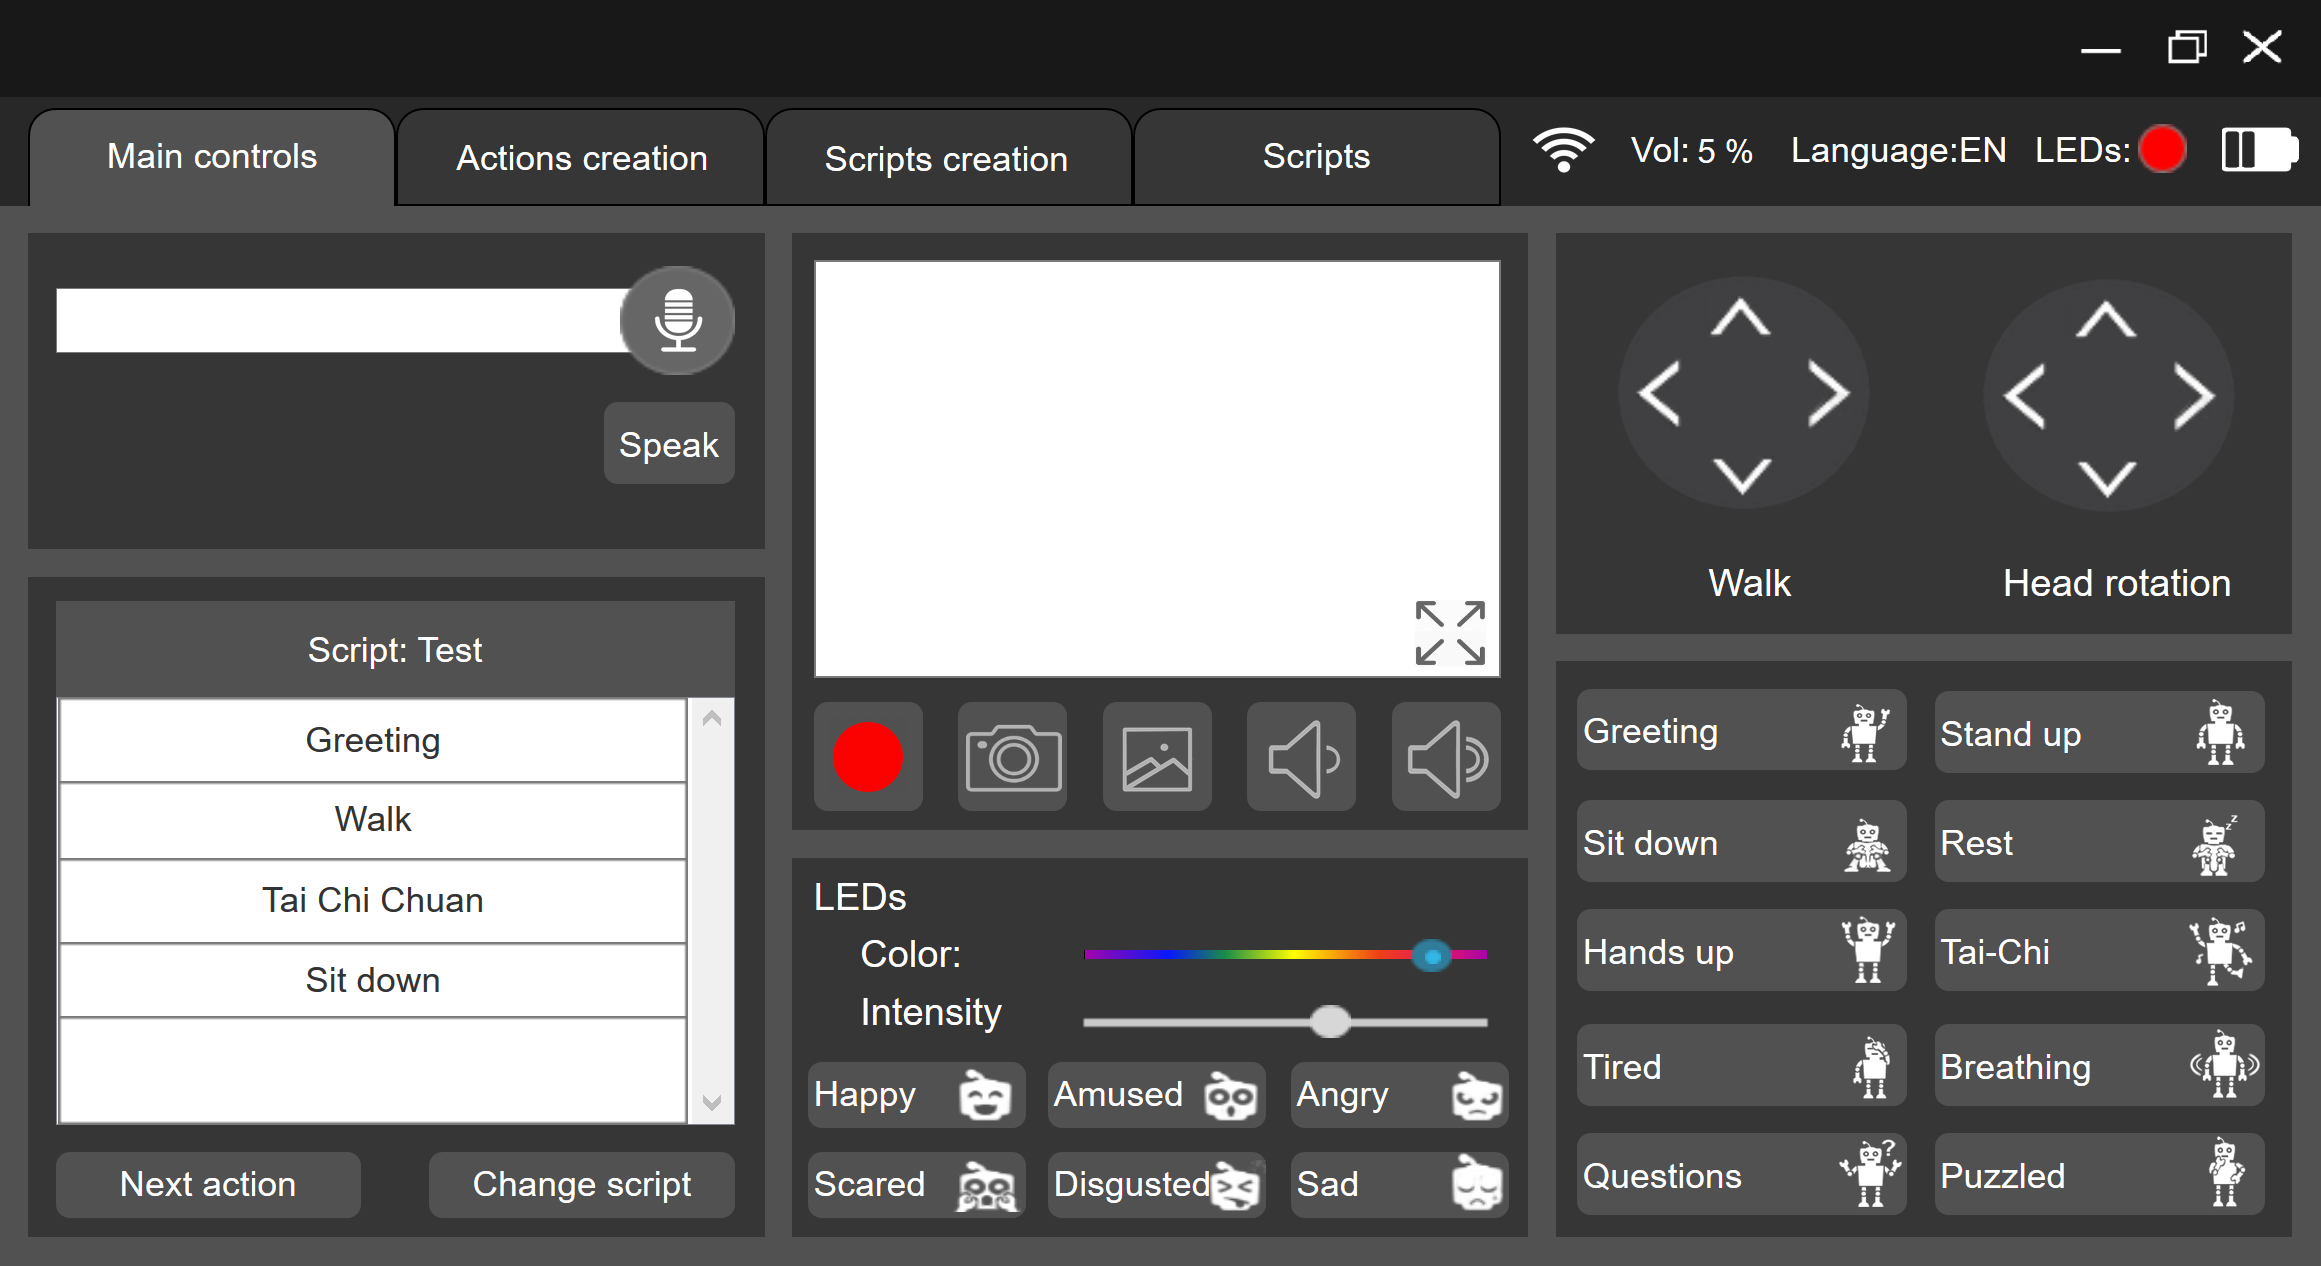
\includegraphics[width=\textwidth]{MainEN.png}
        \caption{Main screen of the interface\label{ref:pantalla1}}
    \end{figure}
    
    As shown in Figure \ref{ref:pantalla1}, the interface's main screen includes the most used actions in a Wizard of Oz role. The top left part shows the speech panel: a way to send the robot words to say, either by typing them or by saying them through a microphone. Below the speech panel, the Script Panel lets the Wizard send previously created actions to the robot in a planned order. The center top section has the camera panel which shows everything the robot is seeing and lets the Wizard capture pictures and video when desired. The center bottom section has the emotion controls for the robot, some colors are associated to emotions according to Johnson \cite{emotion}. 
    Finally, the right panel of the interface contains the movement controls, these allow the Wizard to make the robot walk, move its head and execute prerecorded complex movements.\par
    The interface was developed in Python 2.7 and the 5th version of NAO's operating system.
    Aldebaran's "NAOqi" Python module \cite{aldebaran} was used to give all the functionality to the front-end elements. Multiple sockets where created and used to send movement commands and to receive video and audio for entailing communication between NAO and the wizard's computer. The front-end itself was developed with a python library called "Kivy"\cite{kivy} chosen for its ease to be used and its fast and appealing graphic elements.\par
    
    \begin{thebibliography}{5}
    
        \bibitem{wofoz} J. Bradley \textit{et al}, {\em Wizard of Oz Experiments for Companions}, People and Computers {\bf 23}, 313, 2009
        
        \bibitem{joseiby} J. Hernandez-Cedeño \textit{et al}, {\em NAO as a Copresenter in a Robotics Workshop - Participant’s Feedback on the Engagement Level Achieved with a Robot in the Classroom}, Advances in Human Factors in Robots and Unmanned Systems, 2019, Springer International Publishing.
        
        \bibitem{emotion} D. Johnson \textit{et al}, {\em Imitating Human Emotions with Artificial Facial Expressions}, International Journal of Social Robotics {\bf 5}, 503, 2013
        
        \bibitem{aldebaran} SoftBank Robotics, {\em NAOqi Python - API},  \url{http://doc.aldebaran.com/2-5/ref/python-api.html}, 03-10-2018.
        
        \bibitem{kivy} Kivy Organization {\em Kivy: Cross-platform Python Framework for NUI Development}, \url{https://kivy.org/#home}, 03-10-2018.
        
    \end{thebibliography}

\end{document}
